\section{Estrutura de classes}

Em relação á primeira versão do trabalho, houve e alteraçoes, foram formalizadas classes
para tres camadas da aplicação: domínio (modelo), persistência e API.

A camada do domínio é a que havia sido apresentada antes, com poucas alterações.
A mudança significativa foi a adição de uma nova abstração "PrecoComposto".
Ela foi adicionada porque algumas classes possuiam um método com propósito em comum:
calcular o preço do objeto segundo regras específicas.

A camada de persistência introduziu classes para abstrair a forma como um objeto é persistido.
Foi utilizado o padrão de repositórios, que facilita a extensão gradual da implementação.
Por exemplo, podemos começar usando uma implementação em memória (puro python) e de forma
independente implementar a persistencia com o banco de dados, que é mais complexa.

A camada de API utiliza de uma classe base do framework \href{https://docs.litestar.dev/latest/}{litestart}.
Essas classes são utilizadas para definir os endpoints da API, como listagem, adição ou modificação de recursos. 

\begin{figure}[H]
    \centering
    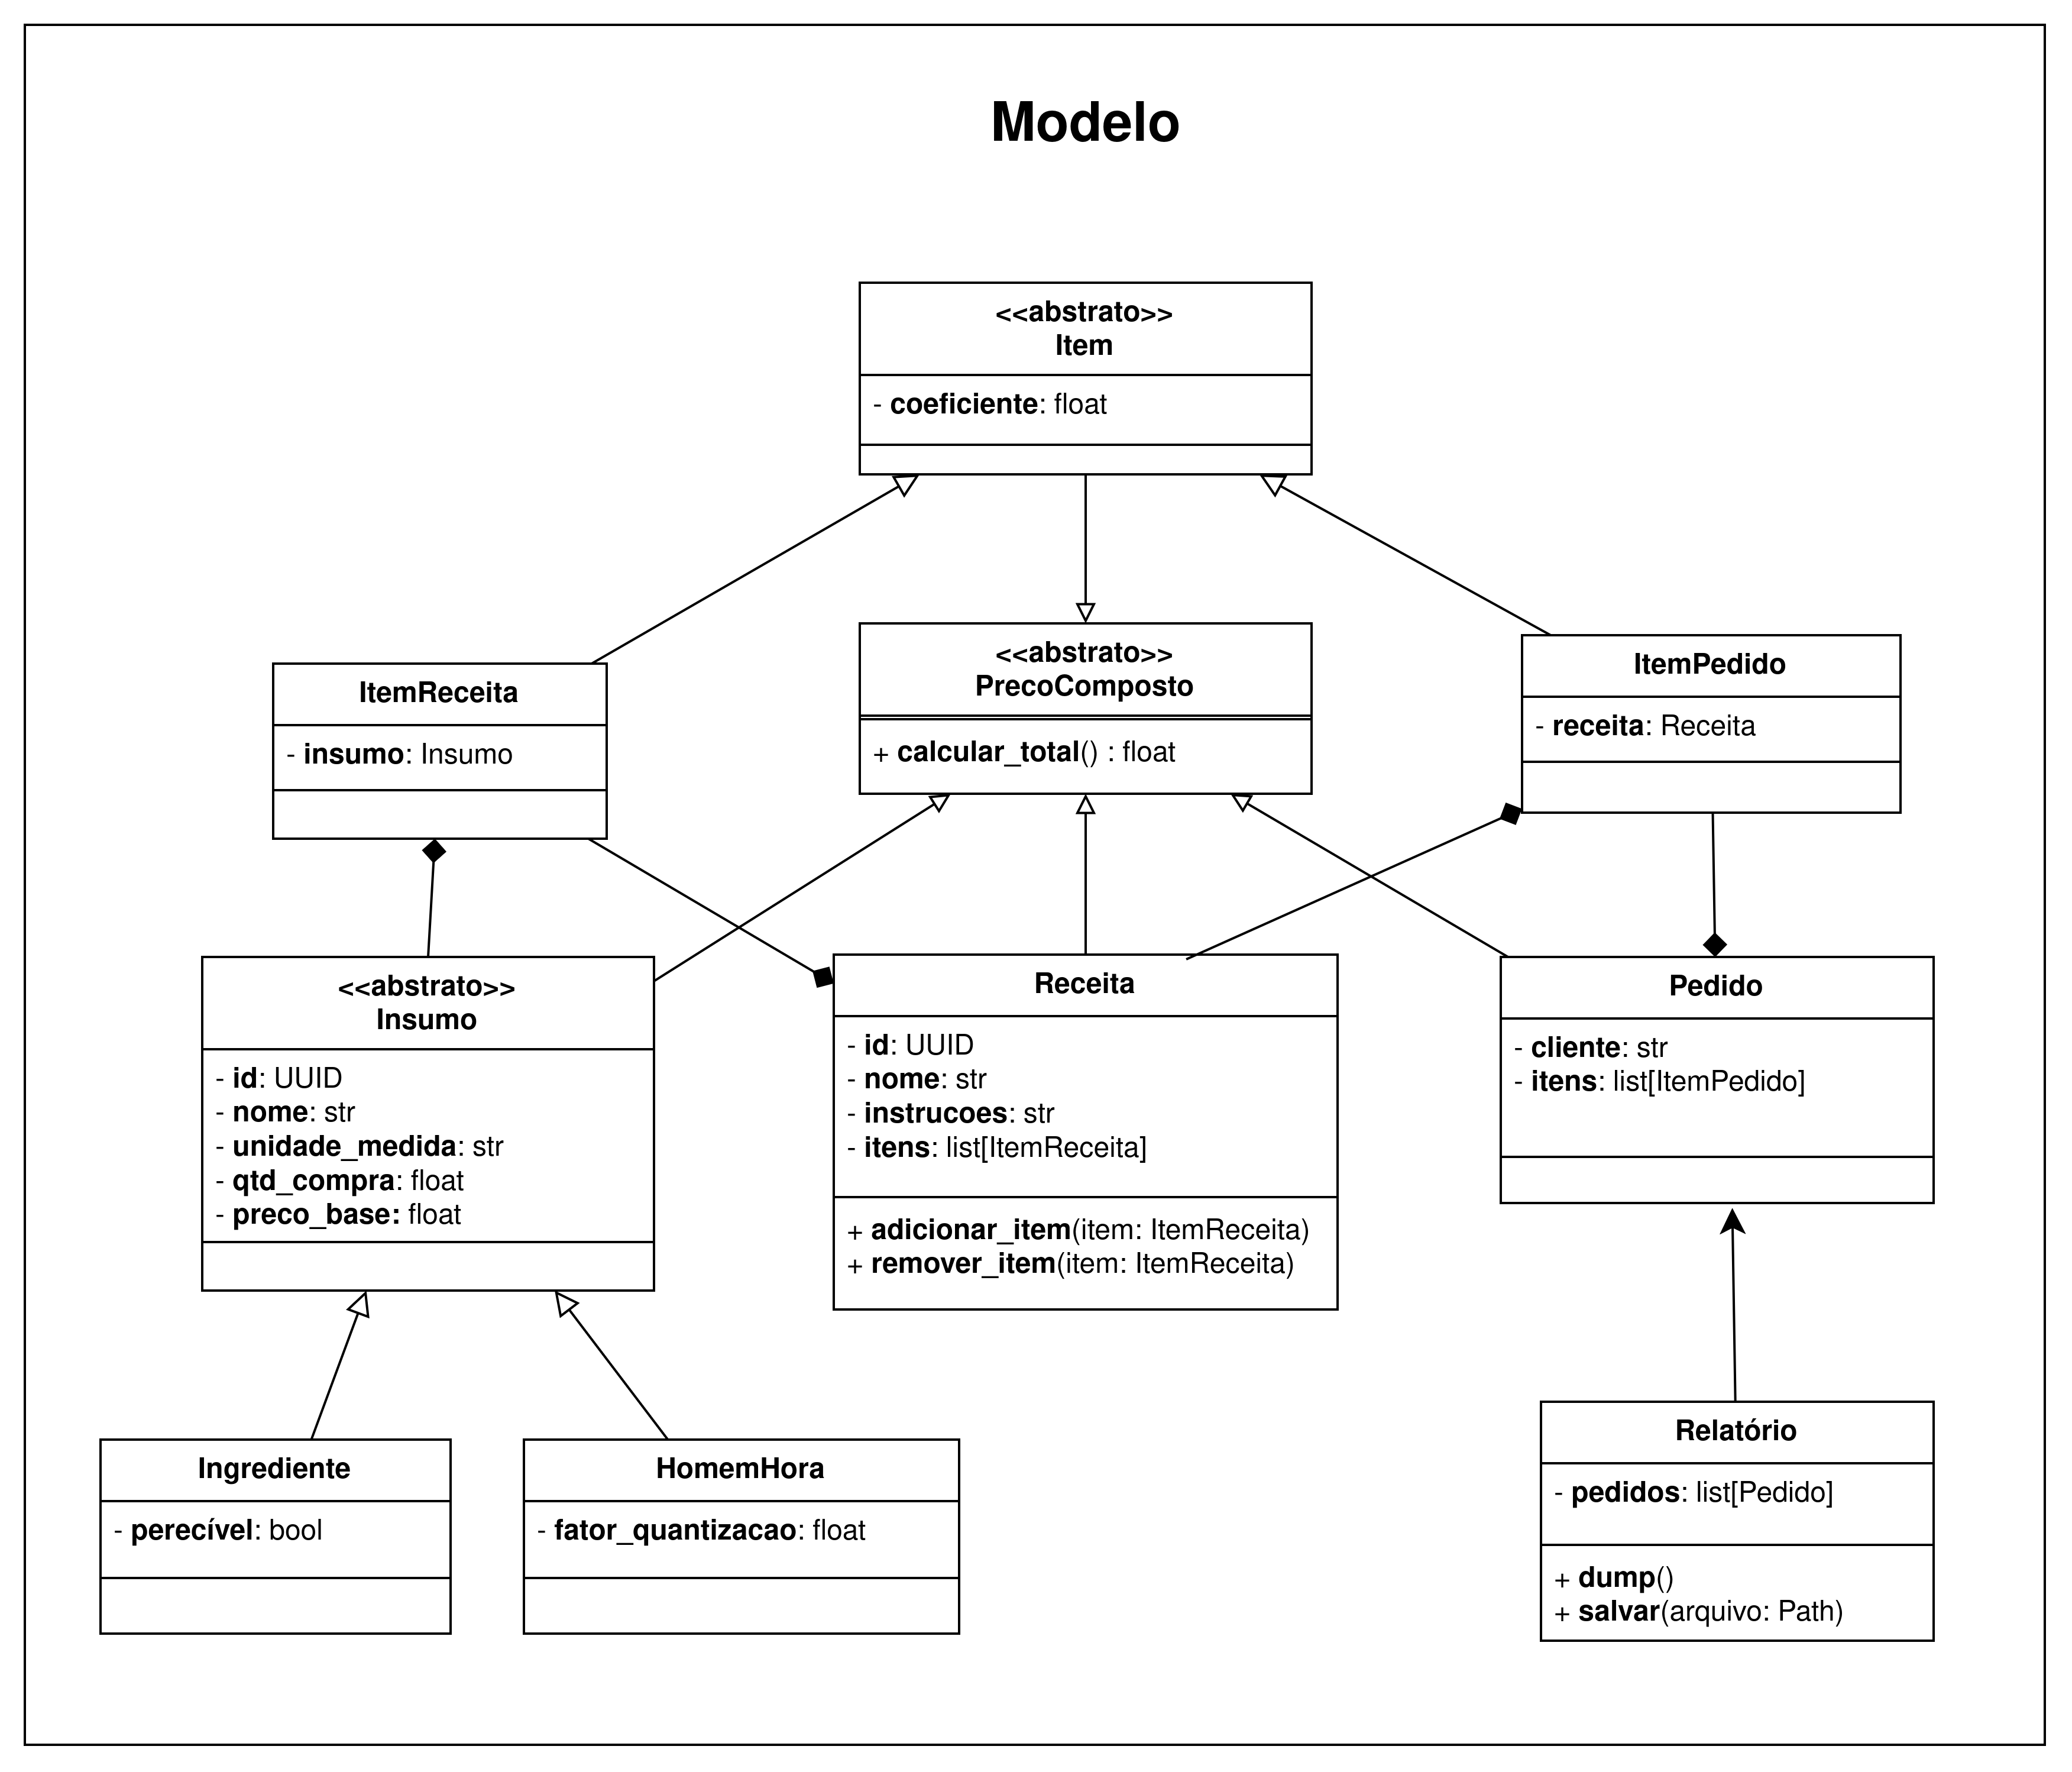
\includegraphics[width=\textwidth]{uml-camada-modelo.png}
    \caption{Camada do domínio}
    \label{fig:uml-modelo}
\end{figure}

\begin{figure}[H]
    \centering
    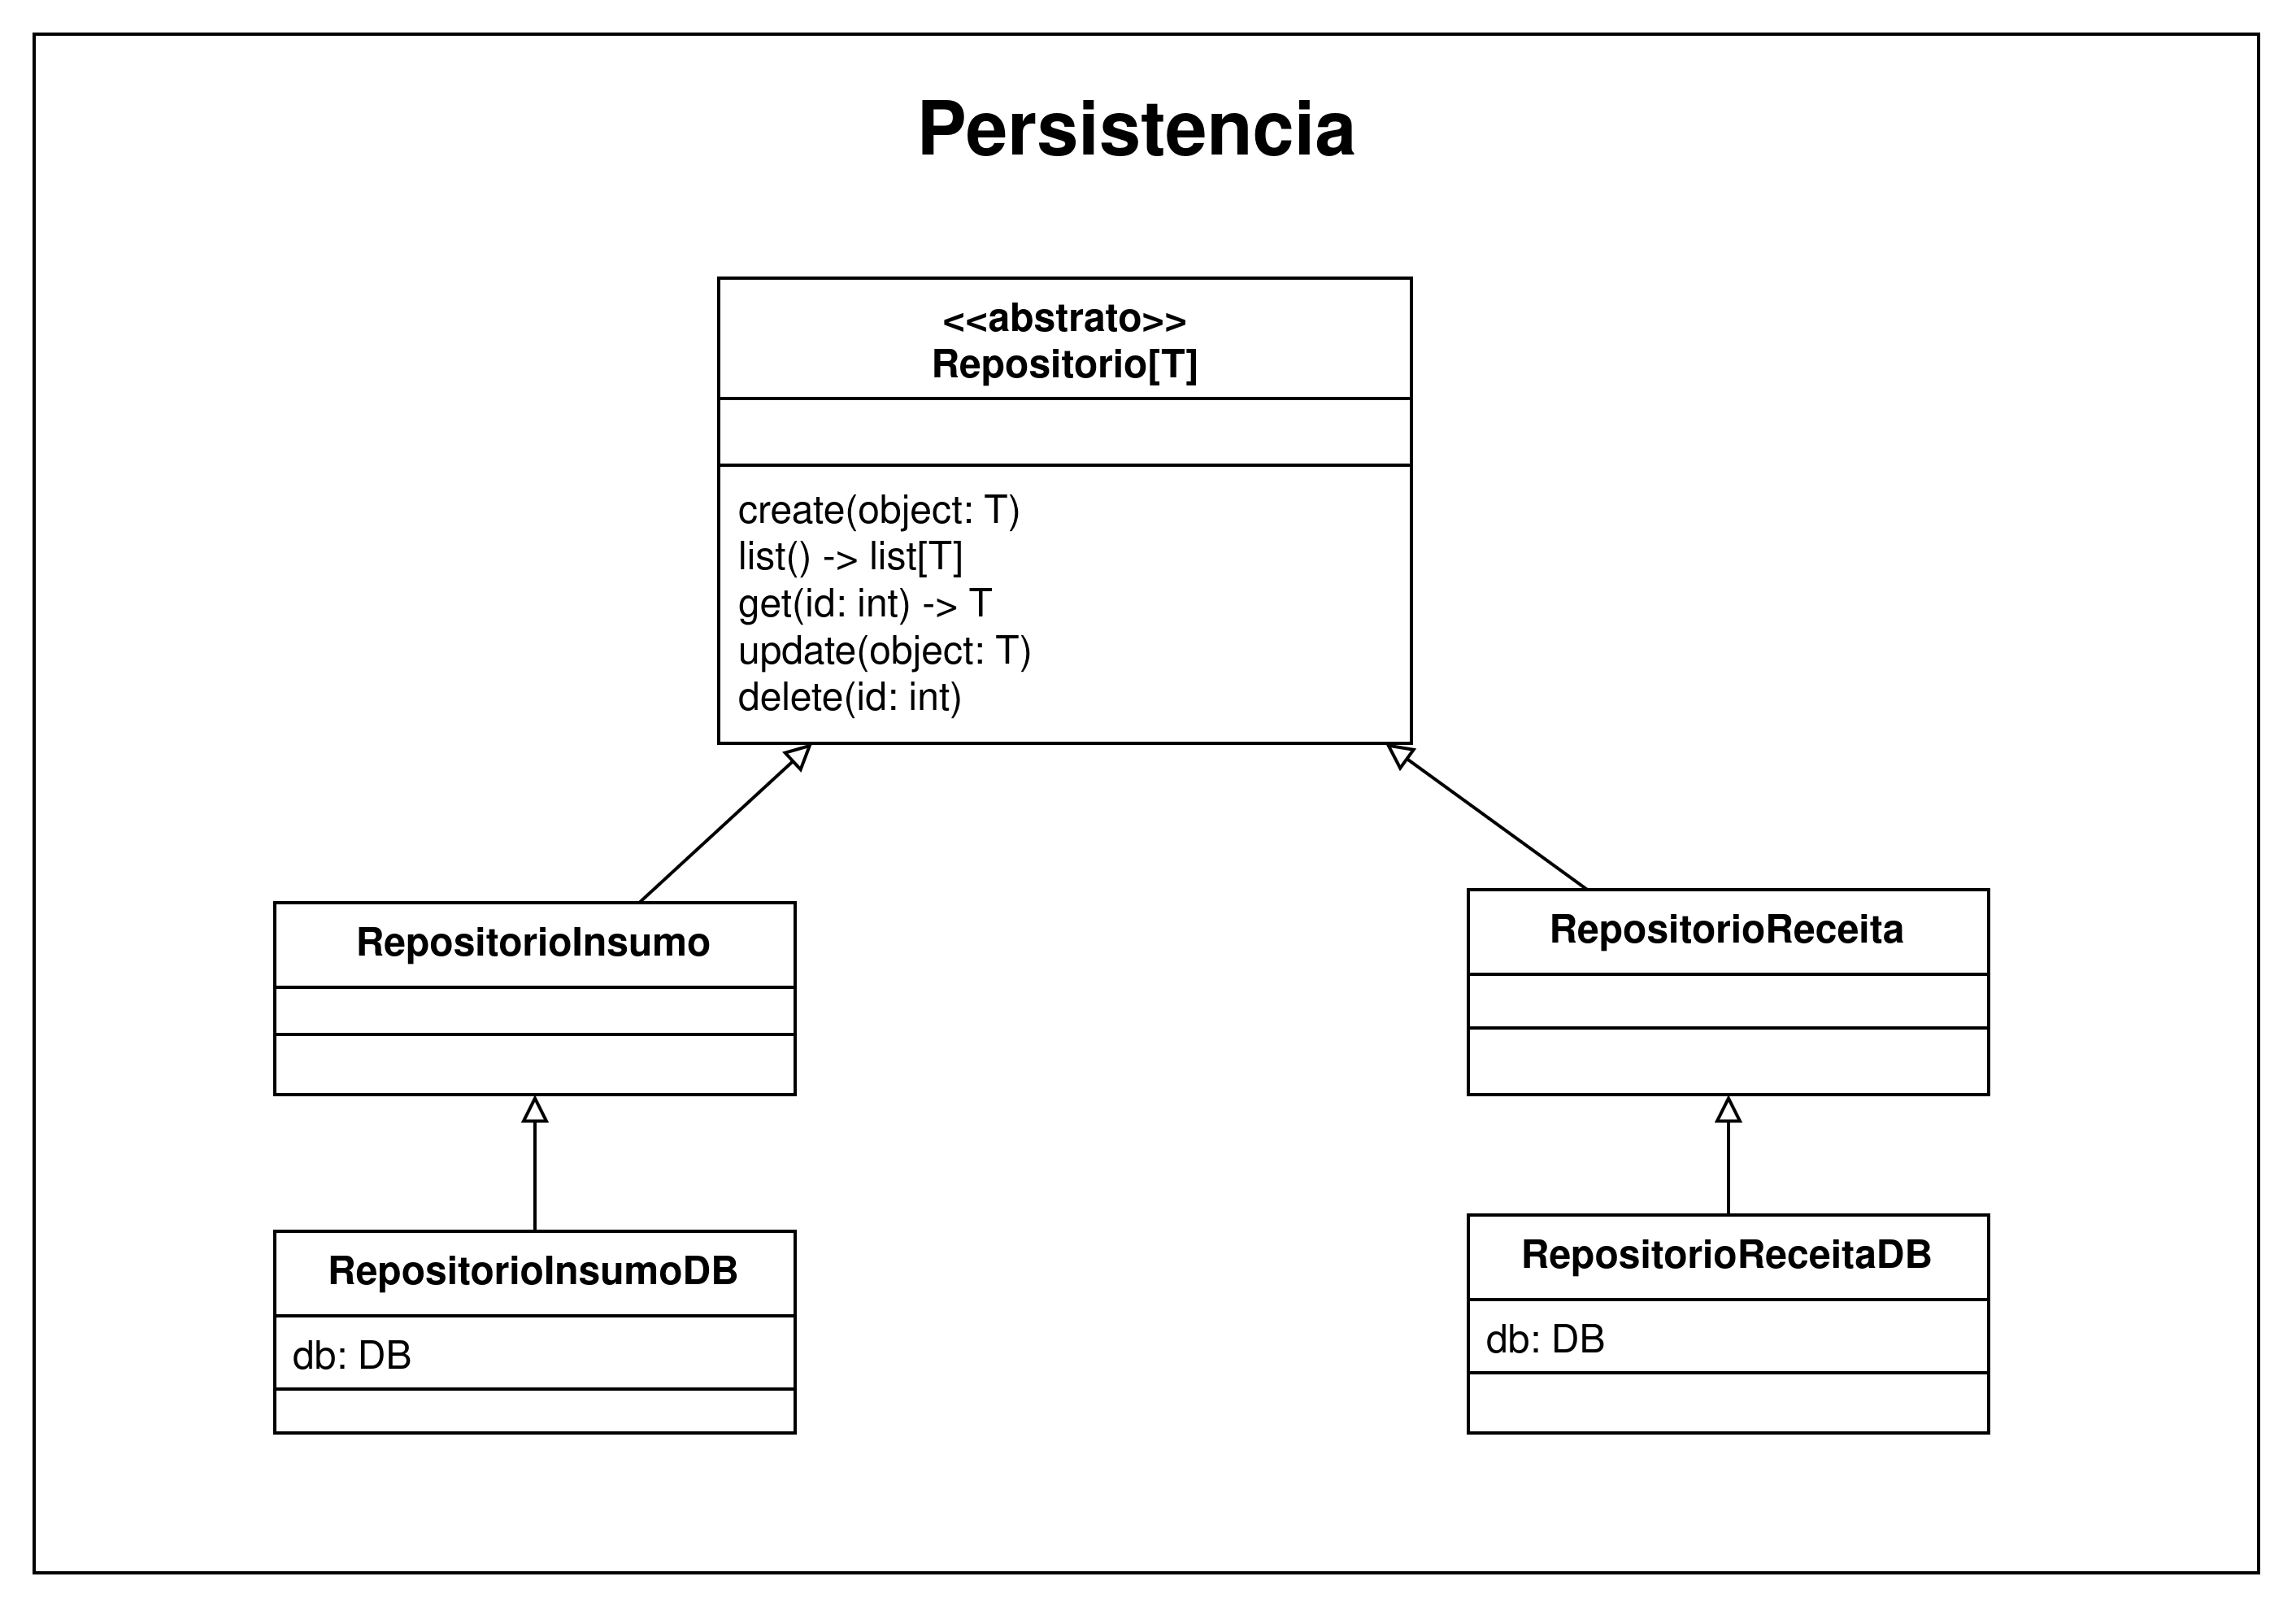
\includegraphics[width=\textwidth]{uml-camada-persistencia.png}
    \caption{Camada de persistencia}
    \label{fig:uml-persistencia}
\end{figure}

\begin{figure}[H]
    \centering
    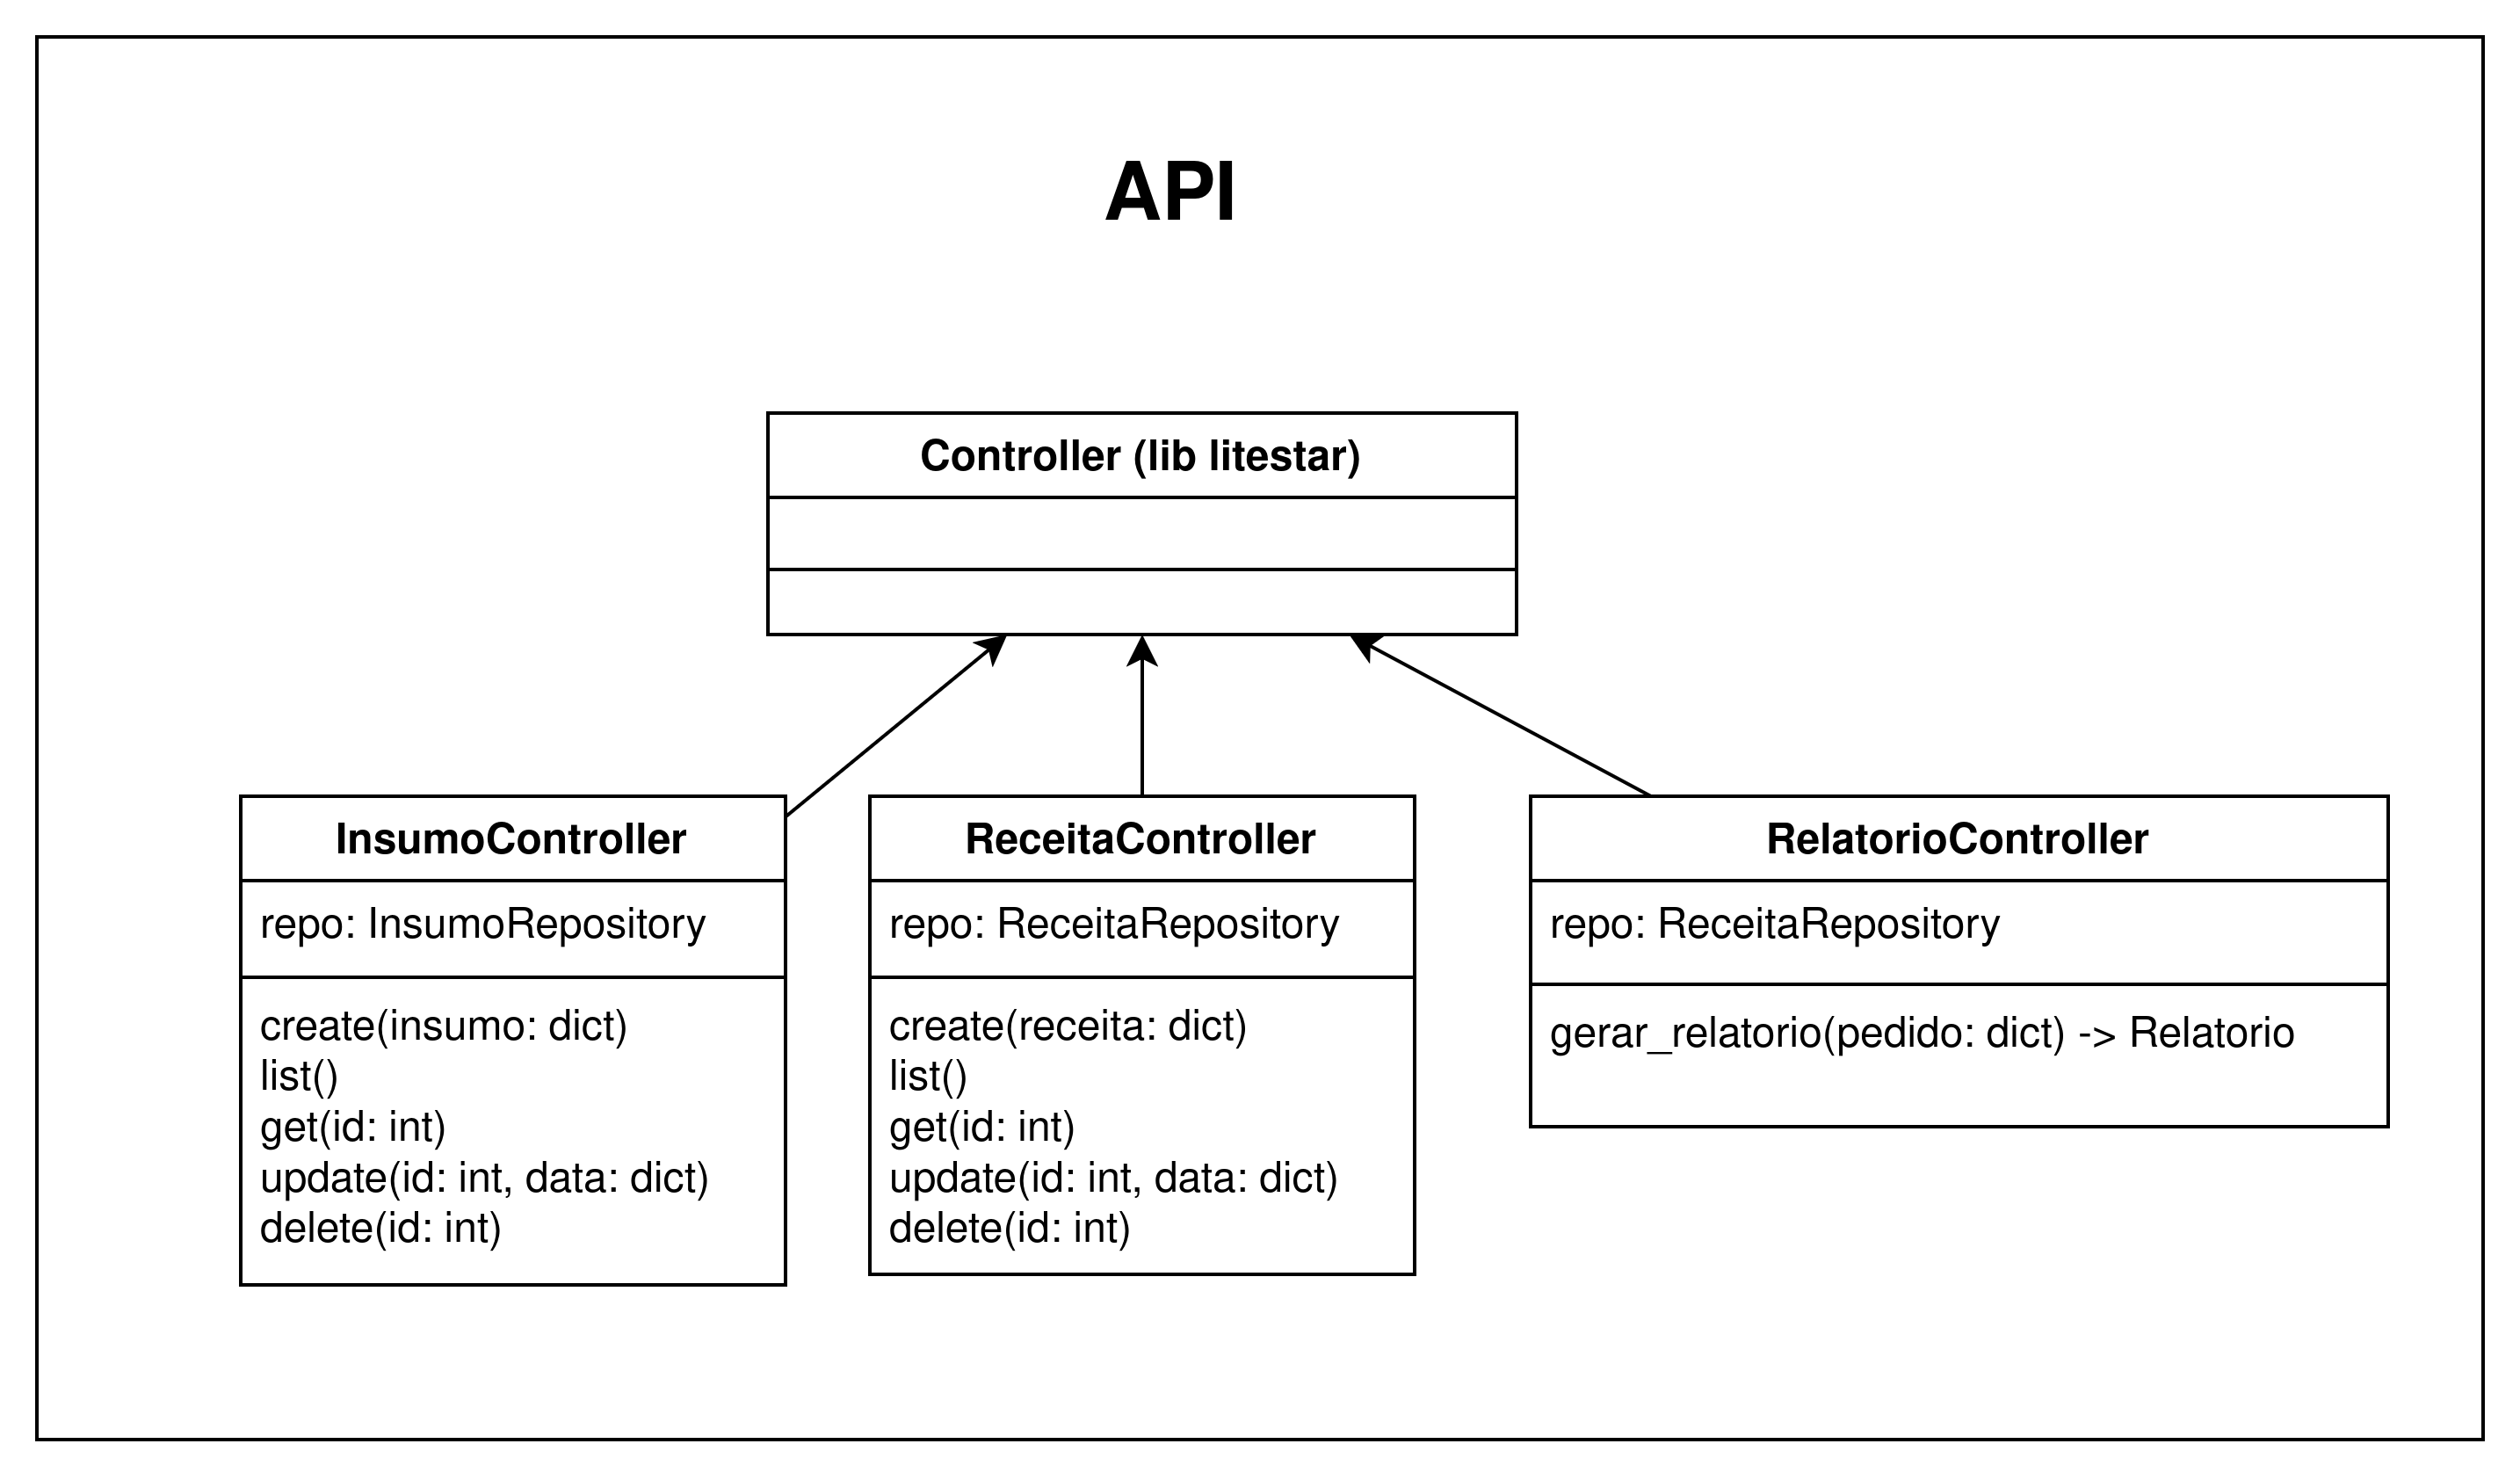
\includegraphics[width=\textwidth]{uml-camada-api.png}
    \caption{Camada de API}
    \label{fig:uml-api}
\end{figure}

\section{Detalhamento}
Nessa seção escolhemos uma funcionalidade principal para detalhar: o cadastro de novos Insumos.

\subsection{Funcionamento}

O cadastro de um novo insumo é iniciado pelo usuário ao enviar uma requisição
\texttt{POST /insumo} com um corpo JSON contendo os campos \texttt{tipo},
\texttt{nome}, \texttt{quantidade}, \texttt{preco\_base} e, quando aplicável,
\texttt{unidade}.

As classes que participam deste processo são:

\begin{itemize}
  \item \texttt{InsumoController} — recebe a requisição e coordena o fluxo;
  \item \texttt{CriarInsumoDTO} — representa e valida a estrutura do corpo da requisição;
  \item \texttt{Ingrediente} ou \texttt{HomemHora} — instanciada de acordo com o campo \texttt{tipo};
  \item \texttt{RepositorioInsumo} — responsável por persistir o objeto criado.
\end{itemize}

Ao receber a requisição, o \texttt{InsumoController} delega a deserialização
do JSON ao \texttt{CriarInsumoDTO}. Com base no campo \texttt{tipo}, o
controlador instancia a classe de domínio correspondente e a repassa ao
\texttt{RepositorioInsumo}, que atribui um identificador único incremental
ao objeto e o armazena em disco. O objeto criado, incluindo o \texttt{id}
gerado, é retornado ao cliente com status \texttt{201 Created}.

\begin{figure}[H]
    \centering
    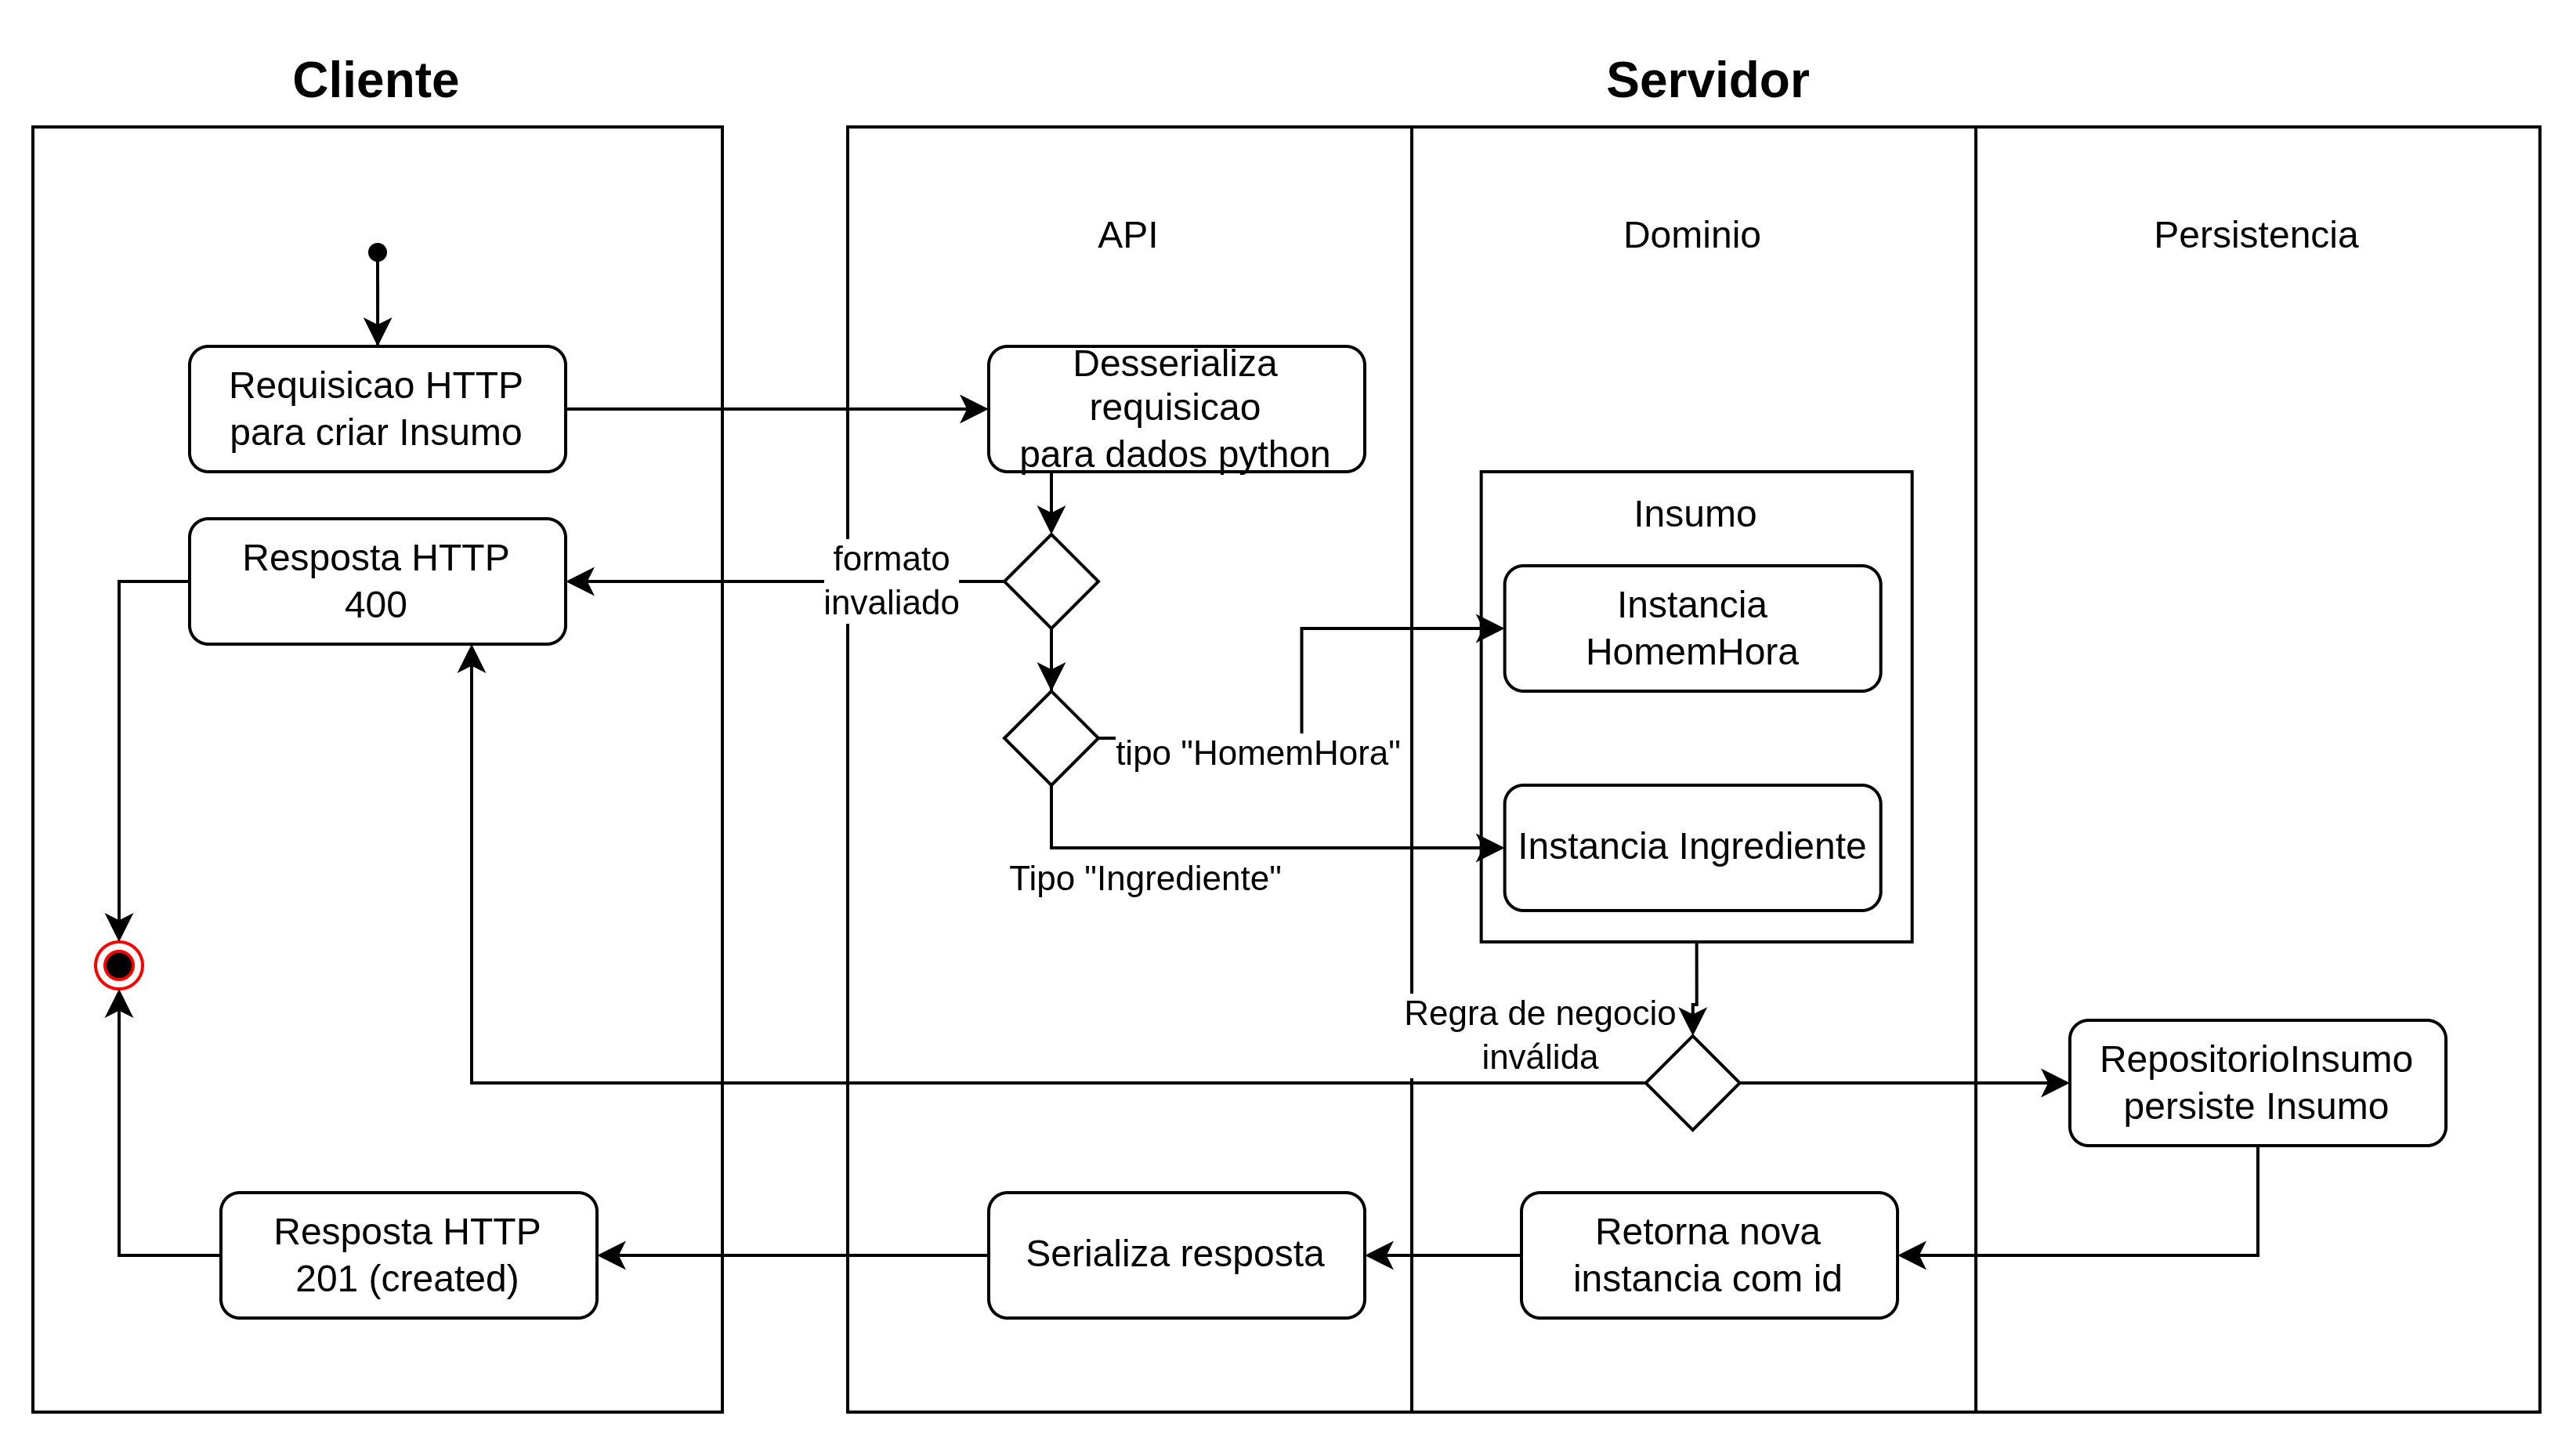
\includegraphics[width=\textwidth]{diagrama-atividade.png}
    \caption{Diagrama de atividades: cadastro de insumo via \texttt{POST /insumo}}
    \label{fig:diagrama-atividades}
\end{figure}

\subsection{Implementação}
Abaixo apresentamos o código implementado para a classe
\texttt{Ingrediente}, que é uma das classes principais do sistema.

\lstinputlisting[
  language=Python,
  caption={Implementação da classe Ingrediente},
  label={list:ingrediente}
]{../../src/projeto_1/dominio/base.py}

\subsection{Saídas do sistema}
Abaixo apresentamos evidências do funcionamento parcial do sistema através de logs de execução.

Os payloads abaixo foram utilizados como entrada nas requisições ao endpoint \texttt{/insumos}.
Os dois primeiros são válidos; os dois últimos ilustram casos de erro.

\lstinputlisting[
  language={},
  caption={Payload válido: criação de Ingrediente},
  label={list:payload-ingrediente}
]{../../examples/post_ingrediente.json}

\lstinputlisting[
  language={},
  caption={Payload válido: criação de HomemHora},
  label={list:payload-homem-hora}
]{../../examples/post_homem_hora.json}

\lstinputlisting[
  language={},
  caption={Payload inválido: tipo desconhecido},
  label={list:payload-tipo-invalido}
]{../../examples/post_tipo_invalido.json}

\lstinputlisting[
  language={},
  caption={Payload inválido: quantidade zero},
  label={list:payload-quantidade-invalida}
]{../../examples/post_quantidade_invalida.json}

\lstinputlisting[
  language={},
  caption={Saída do cliente: requisições e respostas da API},
  label={list:output-client}
]{../../examples/insumo_demo.output_client.txt}

\lstinputlisting[
  language={},
  caption={Saída do servidor: logs do Litestar durante a execução},
  label={list:output-servidor}
]{../../examples/insumo_demo.output_servidor.txt}

\section{Estrutura do Relatório Final}
Abaixo listamos as seções previstas para o relatório final e uma
breve descrição de cada uma.

\begin{itemize}
  \item \textbf{Introdução:} Descrição do contexto e objetivos do projeto.
  \item \textbf{Modelagem:} Detalhamento dos diagramas UML e decisões
    de projeto.
  \item \textbf{Implementação:} Descrição das tecnologias e classes principais.
  \item \textbf{Testes:} Metodologia e resultados da validação do sistema.
  \item \textbf{Conclusão:} Considerações finais sobre o desenvolvimento.
\end{itemize}

\section{Extensabilidade}
Uma possibilidade de expansão futura para este projeto é a adição de outros tipos de insumos, como por exemplo, equipamentos ou materiais consumíveis.
Isso poderia ser feito criando novas classes que herdam de insumo, mas que apresentam características únicas em "receitas" ou "pedidos".

O projeto se inspira muito em CPU(composição de preços unitários), que é uma técnica utilizada na construção civil para precificar serviços, portanto, a adição de outros tipos de insumos é uma extensão natural do projeto.
Neste exemplo, equipamentos pode representar o uso e o custo de uso de máquinas como liquidificadores, fornos, etc.

Já materiais consumíveis podem representar itens que não utilizados para preparar uma receita, mas sim as condições do pedido, como sabão, esponja, embalagens de entrega etc.
A implementação dessas novas classes poderia seguir a mesma estrutura de herança e composição já utilizada para os insumos atuais, facilitando a integração com o sistema existente.
